Fitting the anomalous couplings one at a time while fixing the other couplings
to the Standard Model values, we get the following results:

%% [#1] INFO:Minization --  Including the following contraint terms in minimization: (n_ww_con,n_top_con,n_wjets_con,n_wz_con,n_zz_con,n_dy_con)
%% [#1] INFO:Fitting -- RooAddition::defaultErrorLevel(nll_cpdf_data_with_constr) Summation contains a RooNLLVar, using its error level
%% Minuit2Minimizer: Minimize with max iterations 3500 edmval 1 strategy 1
%% Minuit2Minimizer : Valid minimum - status = 0
%% FVAL  = -1585.15870544803374
%% Edm   = 6.51446699876973863e-06
%% Nfcn  = 141
%% n_dy  = 13.0313 +/-  12.0897(limited)
%% n_top  = 119.079 +/-  38.7019(limited)
%% n_wjets  = 83.4755 +/-  37.2606(limited)
%% n_ww  = 869.599 +/-  68.7677(limited)
%% n_wz  = 18.5447 +/-  3.71087(limited)
%% n_zz  = 10.5946 +/-  1.95429(limited)
%% x_par  = 0.0146317 +/-  0.0555614(limited)
%% Info in <Minuit2>: MnMinos Parameter is at Lower limit. : par = 0
%% Minos:  Parameter  is at Lower limit.
%% Minos: Lower error for parameter 0  :  -10.1063
%% Minos: Upper error for parameter 0  :  13.1768
%% Minos: Lower error for parameter 1  :  -38.9149
%% Minos: Upper error for parameter 1  :  39.0235
%% Minos: Lower error for parameter 2  :  -37.7822
%% Minos: Upper error for parameter 2  :  37.9506
%% Minos: Lower error for parameter 3  :  -68.3564
%% Minos: Upper error for parameter 3  :  69.2349
%% Minos: Lower error for parameter 4  :  -3.72229
%% Minos: Upper error for parameter 4  :  3.72172
%% Minos: Lower error for parameter 5  :  -1.95908
%% Minos: Upper error for parameter 5  :  1.95939
%% Minos: Lower error for parameter 6  :  -0.0621736
%% Minos: Upper error for parameter 6  :  0.033645
%% [#1] INFO:Minization --  Including the following contraint terms in minimization: (n_ww_con,n_top_con,n_wjets_con,n_wz_con,n_zz_con,n_dy_con)
%% [#1] INFO:Fitting -- RooAddition::defaultErrorLevel(nll_cpdf_data_with_constr) Summation contains a RooNLLVar, using its error level
%% Minuit2Minimizer: Minimize with max iterations 3500 edmval 1 strategy 1
%% Minuit2Minimizer : Valid minimum - status = 0
%% FVAL  = -1585.28848536290911
%% Edm   = 2.585748855003718e-05
%% Nfcn  = 145
%% n_dy  = 12.8689 +/-  12.0837(limited)
%% n_top  = 120.652 +/-  38.2499(limited)
%% n_wjets  = 83.1959 +/-  37.2379(limited)
%% n_ww  = 870.183 +/-  68.807(limited)
%% n_wz  = 18.5458 +/-  3.71084(limited)
%% n_zz  = 10.5968 +/-  1.95423(limited)
%% y_par  = 0.0366209 +/-  0.0804761(limited)
%% Info in <Minuit2>: MnMinos Parameter is at Lower limit. : par = 0
%% Minos:  Parameter  is at Lower limit.
%% Minos: Lower error for parameter 0  :  -9.94388
%% Minos: Upper error for parameter 0  :  13.194
%% Minos: Lower error for parameter 1  :  -38.322
%% Minos: Upper error for parameter 1  :  38.7536
%% Minos: Lower error for parameter 2  :  -37.8328
%% Minos: Upper error for parameter 2  :  37.8862
%% Minos: Lower error for parameter 3  :  -68.6391
%% Minos: Upper error for parameter 3  :  69.0298
%% Minos: Lower error for parameter 4  :  -3.72201
%% Minos: Upper error for parameter 4  :  3.72201
%% Minos: Lower error for parameter 5  :  -1.95935
%% Minos: Upper error for parameter 5  :  1.95906
%% Minos: Lower error for parameter 6  :  -0.107619
%% Minos: Upper error for parameter 6  :  0.0578947

%% [#1] INFO:Minization --  Including the following contraint terms in minimization: (n_ww_con,n_top_con,n_wjets_con,n_wz_con,n_zz_con,n_dy_con)
%% [#1] INFO:Fitting -- RooAddition::defaultErrorLevel(nll_cpdf_data_with_constr) Summation contains a RooNLLVar, using its error level
%% Minuit2Minimizer: Minimize with max iterations 3500 edmval 1 strategy 1
%% Minuit2Minimizer : Valid minimum - status = 0
%% FVAL  = -1585.49608456847773
%% Edm   = 0.00016004302809174807
%% Nfcn  = 104
%% n_dy  = 12.836 +/-  12.074(limited)
%% n_top  = 121.683 +/-  38.9333(limited)
%% n_wjets  = 82.1426 +/-  37.3603(limited)
%% n_ww  = 867.974 +/-  68.7172(limited)
%% n_wz  = 18.5414 +/-  3.711(limited)
%% n_zz  = 10.5974 +/-  1.95433(limited)
%% y_par  = -0.0669607 +/-  0.224198(limited)
%% Info in <Minuit2>: MnMinos Parameter is at Lower limit. : par = 0
%% Minos:  Parameter  is at Lower limit.
%% Minos: Lower error for parameter 0  :  -9.91095
%% Minos: Upper error for parameter 0  :  13.1842
%% Minos: Lower error for parameter 1  :  -39.2039
%% Minos: Upper error for parameter 1  :  39.2422
%% Minos: Lower error for parameter 2  :  -37.6457
%% Minos: Upper error for parameter 2  :  38.292
%% Minos: Lower error for parameter 3  :  -68.6146
%% Minos: Upper error for parameter 3  :  68.8813
%% Minos: Lower error for parameter 4  :  -3.71976
%% Minos: Upper error for parameter 4  :  3.72457
%% Minos: Lower error for parameter 5  :  -1.95875
%% Minos: Upper error for parameter 5  :  1.95993
%% Minos: Lower error for parameter 6  :  -0.14722
%% Minos: Upper error for parameter 6  :  0.288082


Systematic uncertainties were included in the fit as Gaussian
constraints.

Final exclusion limits for anomalous couplings are:
\begin{align}
  \lambda_{Z}: [-0.048,0.048]~95\%~\mathrm{C.L.}\\
  \Delta g^{Z}_1: [-0.095,0.095]~95\%~\mathrm{C.L.}\\
  \Delta\kappa_\gamma: [-0.21,0.22]~95\%~\mathrm{C.L.}\\
\end{align}

Figure~\ref{fig:contour} shows 2D confidence limit contour plots for
anomalous couplings.

\begin{figure}[tp]
  \centering
    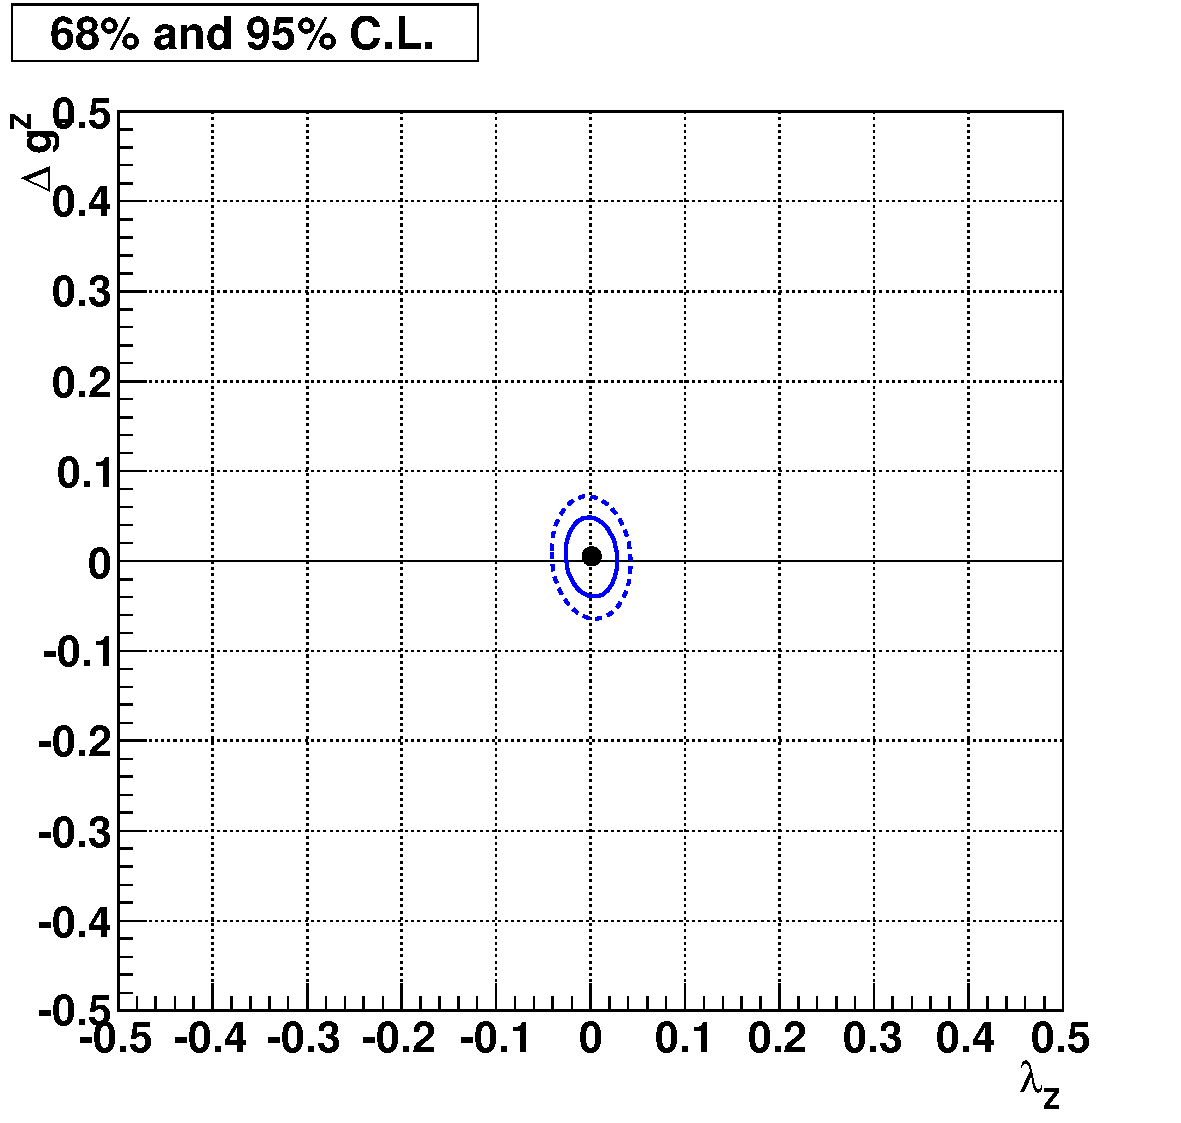
\includegraphics[width=0.7\textwidth]{figures/lz_dgz_contourplot}
    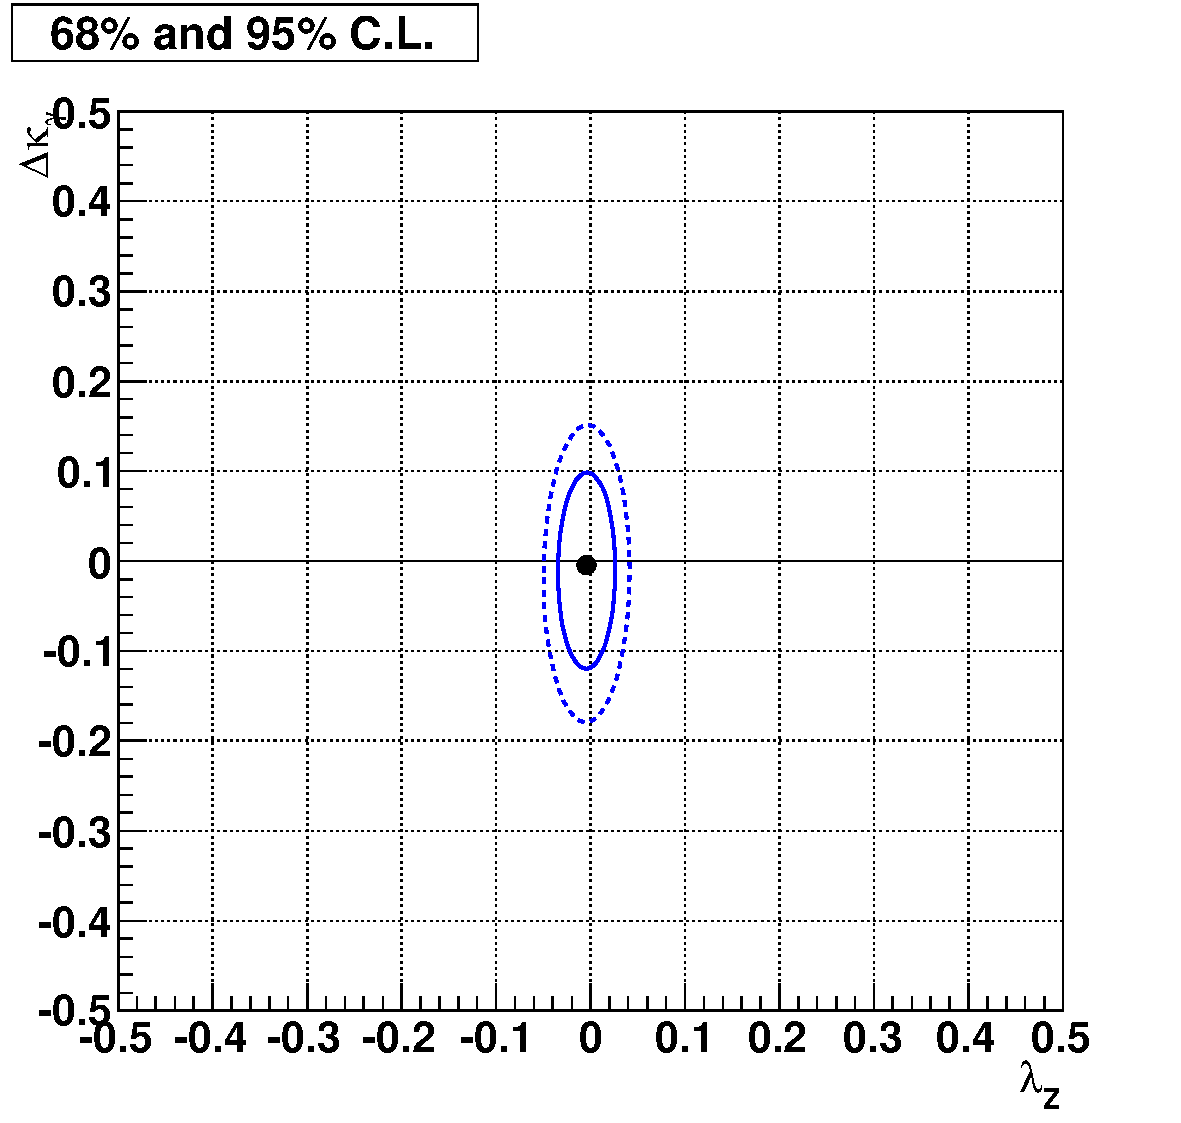
\includegraphics[width=0.7\textwidth]{figures/lz_dkg_contourplot}
  

  \caption[Contour plots for data] {aTGC 68\% and 95\% C.L. contour
    plots for a model without form factors for \intlumi of data.}
  \label{fig:contour}
\end{figure}

